In this chapter, we introduce the basics of quantum computing and reinforcement learning. We start with discussing the basics of the mathematical and computational framework around quantum circuit design. We then describe some algorithms that give quantum computers their advantage.


\section{Quantum Computation}


\subsection{Qubits and Quantum Computation Model}

Quantum Computers store information as quantum bits, or qubits. These qubits can be evolved by operating on them with unitary operators, also called gates. The gate model of computation is rather familiar, following is a diagramatic illustration of the same:

\begin{figure}[h]
    \centering
    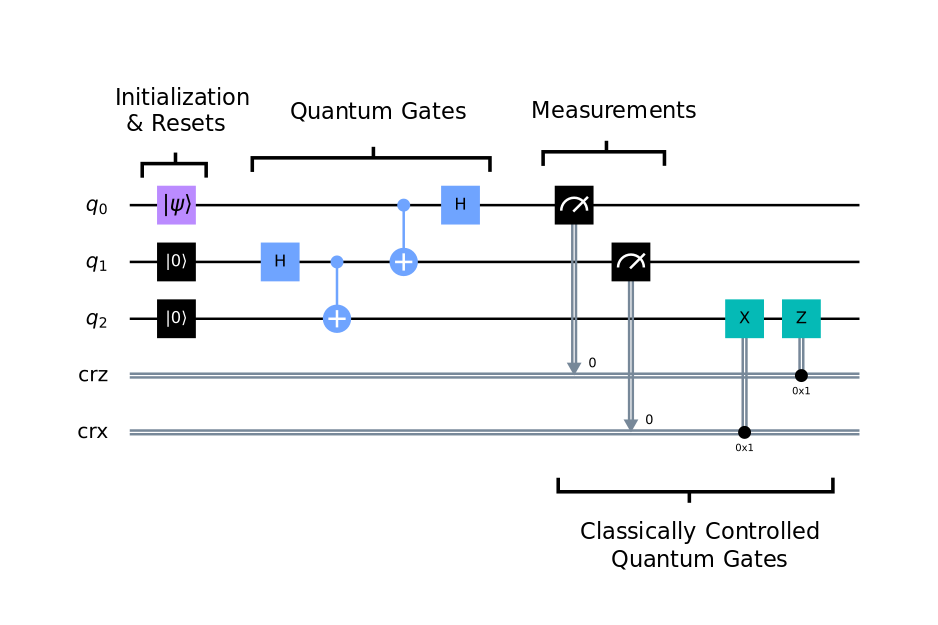
\includegraphics[width=0.8\linewidth]{figures/quantum/quantum_circuit_example.png}
    \caption{The image shows the parts of a typical quantum circuit, with 3 qubits represented by the wires and a set of gates applied to them, followed by measurement of those qubits.}
    \label{fig:quantum-circuit-example}
\end{figure}


A classical bit can be either 0 or 1. However, a qubit can live in any state inbetween 0 or 1, which is understood as being in a weighted superposition of the 0 and 1 states. So the state of a qubit 
\begin{equation}
    \ket{\psi} = \alpha \ket{0} + \beta \ket{1} = \begin{bmatrix}\alpha \\ \beta\end{bmatrix} \;\;\text{such that }\alpha^2 + \beta^2 = 1 \text{ and } \alpha, \beta \in \mathbb{C}
\end{equation}
where the normalization of probabilities forces. However this state of the qubit is not accessible to us, and we can only measure the qubit probabilistically, with probability of being $\ket{0}$ being $\alpha^2$ and that of $\ket{1}$ being $\beta^2$.

Each qubit, in addition to the superposition it is in also has a phase term, which is represented on the bloch-sphere \ref{fig:bloch-sphere} on the x-y plane. The phase doesn't affect the immediate measurement of the qubit, but can affect the resultant phase and superposition when some unitary operation is applied on the qubit.

\begin{figure}[H]
    \centering
    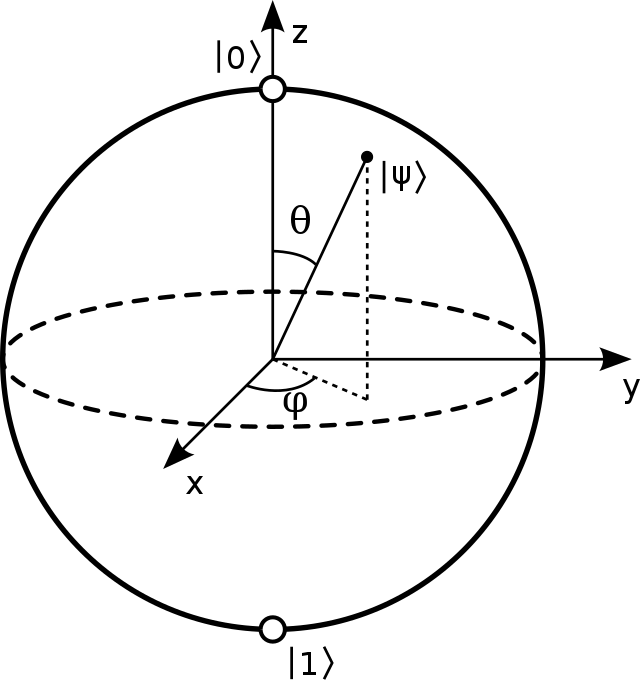
\includegraphics[width=0.5\linewidth]{figures/quantum/bloch_sphere.png}
    \caption{Bloch Sphere represents the state of a qubit $\ket{\psi}$. The pure states $\ket{0}$ and $\ket{1}$ are the vectors along the z-axis on the opposite poles. The angle along the x-y plane represents the phase of the qubits.}
    \label{fig:bloch-sphere}
\end{figure}


\subsection{Unitaries, Gates, and Entanglement}

The state of a system of qubits can be modified by the application of unitary gates on those qubits.

\begin{figure}[h]
    \centering
    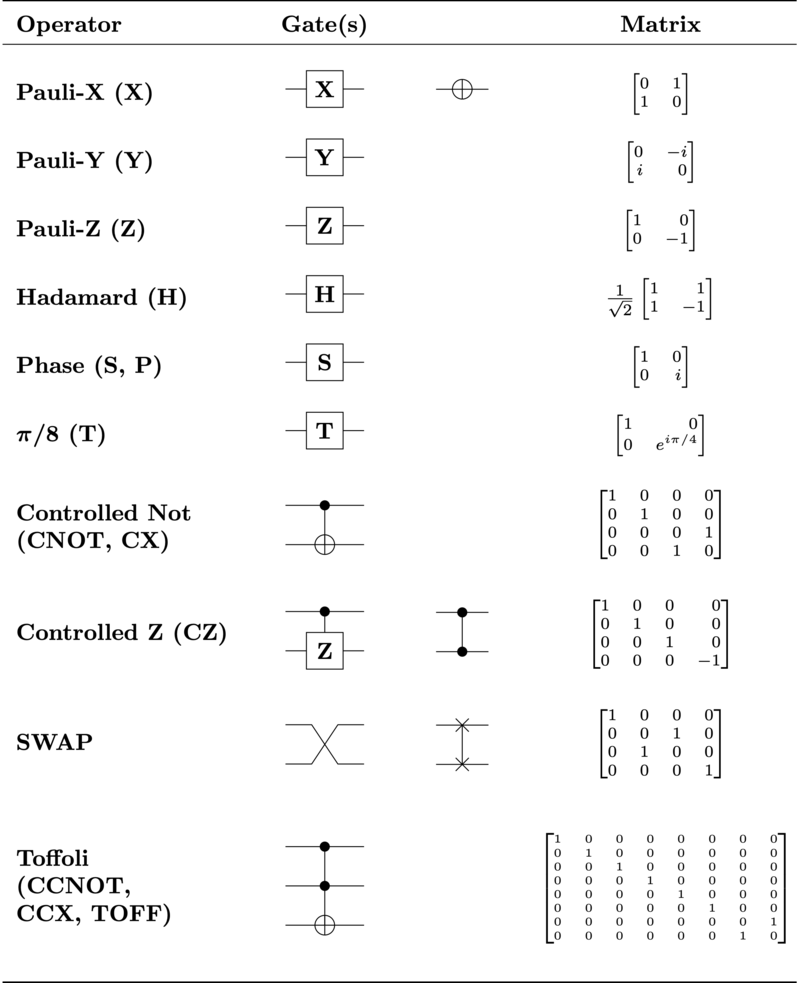
\includegraphics[width=0.7\linewidth]{figures/quantum/quantum_logic_gates.png}
    \caption{Popular logic gates along with their in-circuit representations and corresponding unitary matrices.}
    \label{fig:quantum-unitary-gates}
\end{figure}

Some multi-qubit gates introduce a property called entanglement. Examples of such gates are CNOT, CZ, etc. Once two qubits are ``entangled'' through some such operation like CNOT, their state cannot be written as a product of the individual states of the qubits, their are now linked in a way that the probability distribution of collapsing to either state along th measurement axis is not factorizable. 


\subsection{Density Matrices and Noise}

State preparation on a quantum computer is subject to noise, therefore there often exists some uncertainty in state of qubits on actual physical hardware. This uncertainty can be modelled as a classical probability distribution over the different quantum states that might have been prepared. Such a state is called a mixed state, as opposed to a pure state. Mixed states can be represented using Density matrices $\rho$, which are 2-D matrices with $2^n \times 2^n$ elements for $n$ qubits.
\begin{equation}
    \rho = \sum_{i} p_i \ket{x_i} \bra{x_i}
\end{equation}

Much like unitary operations on state vectors, the application of unitaries on density matrices can be represented through simple matrix multiplication:
\begin{equation}
    \mathcal{O} (\rho) = \sum_i p_i \mathcal{O}(\ket{x_i}) \mathcal{O}(\bra{x_i}) = \sum_i p_i U \ket{x_i} \bra{x_i} U^\dagger = U \rho U^\dagger
\end{equation}


\section{Quantum Algorithms on Error Corrected Computers}

Superposition and Entanglement together provide quantum computers with natural parallel processing power. While full access to this parallelism gets bottlenecked at the measurement layer where we can sample only one of the many states in weighted superposition, it is conceivable that for many an algorithm, this parallelism can result in a processing speed-up. A near-term goal with Quantum Computers is to achieve quantum supremacy, which is to solve a problem (possibly one of no practical use) that no classical computer can solve in a feasible amount of time. \cite{quantum-complexity-survey}


\subsection{Grover's Search}

Grover's search is one of the two most prominent quantum algorithms originally proposed by Grover in 1996 \cite{grover-search-original}, where it was used to solve the problem of searching in a list with no exploitable structure in sub-linear time. Since then, it has been the inspiration for many other algorithms, and many use it as a subroutine call, leading to a class of algorithms called amplitude amplification algorithms \cite{quantum-amplitude-amplification-algorithms}.

\subsubsection{The Problem}

Grover attacks the problem of unstructured search, where we have a list of $n$ elements in an any permutation and we have an oracle which marks each of these elements $1$, which is one of the results of the search procedure we wished to find, or as $0$ which is for those elements which were not one of those elements. We are told that the oracle only returns a value of $1$ for some $m$ of those elements, where $m << n$.

\subsubsection{Overview of the algorithm}

The Algorithm proceeds in two steps:
\begin{enumerate}
    \item \textbf{Preparing the initial superposition of bitstrings:} The initial state should be the superposition of all elements in our search domain. Since these are the indices of the elements we are searching over, we can take this to be an equal superposition of all basis states, constructed by applying the hadamard gate over all qubits.
    \begin{equation}
        \ket{x} = \frac{1}{\sqrt{n}} \sum_{i=1}^{n} \ket{b_i}
    \end{equation}
    \item \textbf{Application of a phase-kickback oracle:} For any input state $\ket{x}$, if it is a valid solution (i.e. $f(x) = 1$), then the oracle that bitstring with a negative phase. If $\ket{x}$ is not a basis state but rather is a superposition of states, then the oracle operates on each basis component of the state independently as shown in equation. \ref{eqn:grover-oracle}
    \begin{equation}\label{eqn:grover-oracle}
        \mathcal{O} \big(\ket{x} \big) = \mathcal{O}\bigg(\sum_i w_i(x) \ket{b_i} \bigg) = \sum_i w_i(x) \begin{cases}
            -\ket{b_i} & \text{if } f(b_i) = 1 \\
            \ket{b_i} & \text{if } f(b_i) = 0
        \end{cases}
    \end{equation}
    \item \textbf{Performing a reflection around the average amplitude:} 
    \item \textbf{Repeat 2 steps above and measure the final state:} We iteratively apply the oracle and the diffuser circuit to take the present superposition closer and closer to the goal state. Measurement of this state along the computational basis gives us a bitstring, which with some constant probability is the solution $x$ such that $f(x) = 1$.
\end{enumerate}

\subsection{Shor's Algorithm}



\section{Hybrid Quantum Classical Algorithms on Near Term Computers}

The algorithms discussed in the section above are not immune to the noise that plagues present day systems, and cannot be feasible run on the quantum computers of today. 


\section{Reinforcement Learning}

\subsection{What is Reinforcement Learning}

Machine Learning and all associated sub-disciplines are motivated by the goal of achieving artificial general intelligence, that is being able to mimic the human mind and even surpass it's capacity to percieve, compute and actuate. The human mind deals with a veritable variety of problems differing greatly in their phrasing, in the solutions they admit, etc. Of this host of problem types, 

Deep Learning is an extremely powerful and popular one of these methods, which uses parameterized function approximators (aka. neural networks) to learn arbitrary functions directly from examples. We typically learn functions which take as input numerical data and associated structure (e.g. graphs) and produce one or many continuous-valued outputs (regression) or discrete-value outputs (classification). This has been employed with great success in computational chemistry, for instance, on predicting properties of molecules like solubility, smell, energy, etc. % Come up with more examples

Despite all their predictive power, these methods are limited in the set of problems they can solve. One limitation is our inability to provide a large number of labeled examples since running laboratory experiments or expensive in-silico simulations are often too time and resource-consuming. Another issue is that the output may not be a simple function of its inputs. For instance, when predicting molecular coordinates from molecular graphs, our outputs depend greatly on each other the position of one atom affects that of all others, and therefore a single step function cannot solve such a problem, an iterative approach to optimize these coordinates is required. In such cases where a problem is solved in many steps, there is no notion of the correct result after a single step, we can only score if the final result is produced by the composite of steps. All these problems necessitate a machine learning method which can produce outputs over several timesteps, and be able to reason about the correctness of its outputs based on rewards it may obtain at a different time in our process. This method is Reinforcement Learning. \cite{rl-intro-sutton-barto}


\subsubsection{Markov Decision Processes}

% What is environment, state, action

A Markov Decision Processes is any real or simulated process going on in time where each each decision follows the Markovian Property, i.e, any future state transitions or rewards are conditionally independent of the past states and actions given the present state the environment is in.

A Markov Decision Process (MDP) can be represented as a tuple $\braket{S, A, T_a(s, s^\prime), R_a(s, s^\prime)}$, where $S$ is the set of all states, $A$ is the set of all actions available from any given state, $T_a(s, s^\prime)$ is the transition model which represents the probability of going from a starting state $s$ to a next state $s^\prime$ given that the action $a$ was taken, and $R_a(s s^\prime)$ is the reward obtained when this transition is realized.

Reinforcement Learning is a method of solving Markov Decision Processes. For our problem to be solved by RL, we need to ensure that our formulation is Markovian, i.e. our state has enough information to, given the action, predict the probability of the next state and the associated reward.

\subsubsection{Value Function and Policy Function}

At every point in time, our agent has access to the state gets to choose an action, for which it gets a reward and the state of the simulation is updated. 
This process continues indefinitely until a terminal state is reached, i.e. one where no further progress needs to be made and no future rewards can be collected. This entire trajectory of states and actions together comprises an episode.

The agent maintains a function which is called it's \textbf{policy function} $\pi(s, a)$, which given the current state gives the probability of each action it can take from that state. Our agent is allowed to be stochastic for various practical and theoretical reasons, so the probability for more than one action in a given state is allowed to be non-zero. This is the function that we shall attempt to optimize while learning from our environment.

While acting according to any policy function, we can associate which each state what we call the \textbf{value function} $V_{\pi}(s)$, which represents the expected sum of rewards till the end of the episode obtainable by following the policy. The optimal policy function $\pi$ is that which leads to the maximum value function for the starting state.

Value-function of one state can be written in terms of that of others, and to compute these values over all the states we need to iteratively apply our updates.

\begin{equation}
    V(s) = \sum_{a \in A} \pi(s, a) \sum_{s^\prime} T_a(s, s^\prime) (V(s^\prime) + R_a(s, s^\prime))
\end{equation}

Instead of associating a value with each state, we can associate it with a state-action pair. This function is called the Q-function, and it carries equivalent information to the value function.
\begin{eqnarray}\label{eqn:defn-q-v-fn}
    Q(s, a) &=& \sum_{s^\prime} T_a(s, s^\prime) \bigg(R(s, s^\prime) + V(s^\prime) \bigg)\\
            &=& \sum_{s^\prime} T_a(s, s^\prime) \bigg(R(s, s^\prime) + \sum_{a \in A} \pi(s^\prime, a) Q(s^\prime, a)\bigg)
\end{eqnarray}

\subsection{Reinforcement Learning Algorithms}

In the following sections, we shall see three kinds of models:
\begin{itemize}
    \item Value Function Optimizers
    \item Policy Function Optimizers
    \item Actor-Critic Systems
    \item Planning based Reinforcement Learning
\end{itemize}


\subsubsection{Deep Q-Networks}

The first class of models attempt to approximate the value function. Assuming that our policy function will be that which is optimal, and assuming that our actions are deterministic (i.e. transition probabilities are 1 for the state we result in after an action and 0 otherwise), we can rewrite equation \ref{eqn:defn-q-fn} as:
\begin{eqnarray}\label{eqn:defn-q-fn}
    Q(s, a) \leftarrow R(s, s^\prime) + \max_{a \in A} Q(s^\prime, a)
\end{eqnarray}

For almost all problems in the real world, the state space is too large to maintain explicitly. Therefore we use a parameterized function $Q_{\theta}$, typically a neural network, to approximate the q-value from any given state-action pair.

The parameters $\theta$ can be updating using gradient based methods. The update operation in equation \ref{eqn:q-update} is 
\begin{equation}
    \label{eqn:q-update}
    \begin{split}
        \theta_{k+1} = \theta_k - \alpha \nabla_\theta \Bigg[\frac{1}{2} \bigg(Q_\theta(s, a) - \Big(R(s, a, s^\prime) + \gamma \max_{a^\prime} Q_{\theta_k}(s^\prime, a^\prime)  \Big) \bigg) \Bigg] \Bigg\vert_{\theta_k}
    \end{split}
\end{equation}

Several improvements to the training efficiency and stability to the DQN algorithm have been made, a few examples are the Double DQN by \cite{double-dqn}. These set of improvements put together have been analyzed by \cite{rainbow-dqn} under the name Rainbow DQN.

\subsubsection{Policy Function Approximators}

The policy function $\pi_\theta(s, a)$ gives the probability of each action given the state. In value function methods, we computed the policy by finding the action with the maximum expected value and assigning it a probability of 1 and other actions 0 for each state. When learning the policy directly, we use a stochastic policy instead, which makes the choice of actions smooth and optimizable.

\paragraph{Reasons to use policy gradients:}
\begin{enumerate}
    \item Learning value function may be much harder than learning the relative quality of actions, e.g. given the task of designing molecules with high solubility, and a procedure which keeps adding bonds iteratively, it can be very hard to predict the expected solubility of the molecule formed at the end of trajectories (value function), while predicting that adding a highly polar bond is more beneficial than adding non-polar ones (policy function).
    \item We might want to obtain a policy which is inherently stochastic, where policy based methods are the better choice. One example is when designing molecules with certain properties, we want a stochastic policy so that we can sample different molecules that optimize on the target property and then rank them based on synthetic ease or the such.
    \item Many a times, the action space is continuous or intractably large, and maximizing value over all actions is not feasible. Here we can only use policy based methods. Geometry optimization is one example, where the action is predicting the molecular coordinates of a single atom, which leads to a un-countably infinite sized action space.
\end{enumerate}

\paragraph{Method:}
To optimize our policy, we sample trajectories from our policy and increase the probability of actions in trajectories which high reward get increase, and those with lower reward decrease.

The utility of our policy is the expected reward under trajectories sampled from this policy, this is the quantity we wish to maximize over the parameters $\theta$. To perform this maximization, we compute $\nabla_\theta U(\theta)$ and update the parameter vector as $\theta \leftarrow \theta + \epsilon \nabla_\theta U(\theta)$. The gradient only depends on the gradient of the log of our policy function scaled by the rewards obtained along the trajectory, and very importantly does not depend on the true transition model. Equation \ref{eqn:policy-grad} follows from a mathematically involved derivation done in \cite{}.

\begin{equation}\label{eqn:policy-grad}
    \nabla_\theta U(\theta) \leftarrow \frac{1}{m} \sum_{i=1}^{m} \sum_{t=0}^{H-1} \nabla_\theta \log \pi_\theta (u_t^{(i)}|s_t^{(i)}) \Bigg(\sum_{k=t}^{H-1} R(s_k^{(i)}, u_k^{(i)}) - b(s_t^{(i)})\Bigg)
\end{equation}

\paragraph{Other Nuances:} Despite having the gradient that we need to update along, it's unclear what learning rate we should use to perform said update. Unlike in deep learning where the next iteration would correct if we overstep along the gradient, an overstep in our policy can lead to evaluation over an incorrect policy and can essentially wipe out all we have learnt till now. Trust Region policy optimizations (TRPO) by \cite{trpo} and Proximal Policy Optimizations (PPO) by \cite{ppo} are methods that address this. Furthermore, to increase sample efficiency, Direct Deterministic Policy Gradients (DDPG) by \cite{ddpg} and Soft Actor critic (SAC) \cite{sac} are used. These methods have not seen great application in chemistry but hold great promise given their popularity in other reinforcement learning sub-domains.

\subsubsection{Actor Critic Methods}

In equation \ref{eqn:policy-grad}, we are free to subtract a baseline value $b(s_t^{(i)})$ from the summed up rewards for each action, however this baseline should be independent of the action and can only depend on the state. Subtraction of this baseline leads to lower variance estimates in the value of actions. The network for each action now has to predict a quantity called the advantage, which represents the relative value of the actions and abstracts out the value of the state.
\begin{equation}\label{eqn:advantage}
    A(s, a) = Q(s, a) - V(s)
\end{equation}

This is implemented in practice using two networks, an actor network, which estimates the values of the actions, and a critic network, that estimates the resultant values of the states which we subtract as baseline from the rewards. These methods are often known to be stabler than their pure policy-gradient counterparts.

There are several variants on how the critic network and the explicit rollout together lead to the estimate of the value for each state, which have been discussed in detail by \cite{actor-critic-a2c, actor-critic-a3c, actor-critic-gae}

\subsubsection{Monte Carlo Tree Search}

When the transition model (next state and reward given action) is known, we can plan explicitly using a tree search. Since tree would grow combinatorially big (molecule generation via such means would have every possible molecule and it's substructure as a node in the tree), we use reinforcement learning to find out the most promising nodes. Monte Carlo Tree Search is one such method, which has gained prominence due to it's use in AlphaGo by \cite{mcts-alphago} to play Go and in AlphaZero by \cite{mcts-alphazero} to play Chess, Go, and other games with no human supervision during training. 

MCTS has been used in extensively chemistry wherever the exact transition model is known, in problems like Molecule Generation and Reaction path prediction. 



% Progress in computational techniques and speed is intimately tied to the furtherance of scientific inquiry. Over the past many decades, we have built computers that can simulate systems better and search for courses of action to modify the evolution of these systems to human advantage. In this endeavor, the manifold increase in computational speed and memory has helped us to date, but now that computational components have reached the size of atoms, we seem to be on the verge of meeting a hard limit. Therefore, we have started to look towards other paradigms to develop computers more suited to performing simulations of nature. Quantum computing, the idea of using the fundamental quantum nature of the universe to simulate itself but in much greater generality, has held the most promise.

% Richard Feynman said: “Nature isn't classical, dammit, and if you want to make a simulation of nature, you'd better make it quantum mechanical, and by golly it's a wonderful problem, because it doesn't look so easy.” \cite{feynman-quantum-simulating-physics}

% Though Quantum Computers are realizable even today, the devices in the present day are said to be a part of the Noisy Intermediate-Scale Quantum era (NISQ). Presently, the quantum bits and operations are noisy and lack the reliability to perform any computation infeasible on classical computers of the day.
